\documentclass{article}\usepackage{graphicx, color}
%% maxwidth is the original width if it is less than linewidth
%% otherwise use linewidth (to make sure the graphics do not exceed the margin)
\makeatletter
\def\maxwidth{ %
  \ifdim\Gin@nat@width>\linewidth
    \linewidth
  \else
    \Gin@nat@width
  \fi
}
\makeatother

\IfFileExists{upquote.sty}{\usepackage{upquote}}{}
\definecolor{fgcolor}{rgb}{0.2, 0.2, 0.2}
\newcommand{\hlnumber}[1]{\textcolor[rgb]{0,0,0}{#1}}%
\newcommand{\hlfunctioncall}[1]{\textcolor[rgb]{0.501960784313725,0,0.329411764705882}{\textbf{#1}}}%
\newcommand{\hlstring}[1]{\textcolor[rgb]{0.6,0.6,1}{#1}}%
\newcommand{\hlkeyword}[1]{\textcolor[rgb]{0,0,0}{\textbf{#1}}}%
\newcommand{\hlargument}[1]{\textcolor[rgb]{0.690196078431373,0.250980392156863,0.0196078431372549}{#1}}%
\newcommand{\hlcomment}[1]{\textcolor[rgb]{0.180392156862745,0.6,0.341176470588235}{#1}}%
\newcommand{\hlroxygencomment}[1]{\textcolor[rgb]{0.43921568627451,0.47843137254902,0.701960784313725}{#1}}%
\newcommand{\hlformalargs}[1]{\textcolor[rgb]{0.690196078431373,0.250980392156863,0.0196078431372549}{#1}}%
\newcommand{\hleqformalargs}[1]{\textcolor[rgb]{0.690196078431373,0.250980392156863,0.0196078431372549}{#1}}%
\newcommand{\hlassignement}[1]{\textcolor[rgb]{0,0,0}{\textbf{#1}}}%
\newcommand{\hlpackage}[1]{\textcolor[rgb]{0.588235294117647,0.709803921568627,0.145098039215686}{#1}}%
\newcommand{\hlslot}[1]{\textit{#1}}%
\newcommand{\hlsymbol}[1]{\textcolor[rgb]{0,0,0}{#1}}%
\newcommand{\hlprompt}[1]{\textcolor[rgb]{0.2,0.2,0.2}{#1}}%

\usepackage{framed}
\makeatletter
\newenvironment{kframe}{%
 \def\at@end@of@kframe{}%
 \ifinner\ifhmode%
  \def\at@end@of@kframe{\end{minipage}}%
  \begin{minipage}{\columnwidth}%
 \fi\fi%
 \def\FrameCommand##1{\hskip\@totalleftmargin \hskip-\fboxsep
 \colorbox{shadecolor}{##1}\hskip-\fboxsep
     % There is no \\@totalrightmargin, so:
     \hskip-\linewidth \hskip-\@totalleftmargin \hskip\columnwidth}%
 \MakeFramed {\advance\hsize-\width
   \@totalleftmargin\z@ \linewidth\hsize
   \@setminipage}}%
 {\par\unskip\endMakeFramed%
 \at@end@of@kframe}
\makeatother

\definecolor{shadecolor}{rgb}{.97, .97, .97}
\definecolor{messagecolor}{rgb}{0, 0, 0}
\definecolor{warningcolor}{rgb}{1, 0, 1}
\definecolor{errorcolor}{rgb}{1, 0, 0}
\newenvironment{knitrout}{}{} % an empty environment to be redefined in TeX

\usepackage{alltt}
% !Rnw weave = knitr
% sweave fig help:
% http://users.stat.umn.edu/~geyer/Sweave/foo.pdf
% borrowing design from roxygen -- AJB Jan 13

%% \VignetteIndexEntry{An overview of rlpSpec.}
%% \VignetteEngine{knitr}

\usepackage[utf8]{inputenc}
\usepackage{fancyvrb}
\usepackage[pdfborder={0 0 0}]{hyperref}
\usepackage{url}
\usepackage{upquote}
\usepackage{graphicx}
\usepackage{grffile}
\usepackage{float}
\usepackage{natbib}
\usepackage{amsmath}
\usepackage{geometry}
\geometry{verbose,tmargin=3cm,bmargin=5cm,lmargin=2.5cm,rmargin=2.5cm}
%\usepackage{fullpage}
%captions
\usepackage[font=sf, labelfont={sf,bf}, margin=2cm]{caption}
\usepackage{makeidx} % for indexing
%\usepackage{showidx} % shows page (remove when complete)
\makeindex % comment to have no index
%
\newcommand{\SC}[1]{\textsc{#1}}
\newcommand{\SCY}[0]{\SC{Yes}}
\newcommand{\SCN}[0]{\SC{No}}
\newcommand{\Rcmd}[1]{\texttt{#1}}
\newcommand{\rlp}[0]{\Rcmd{rlpSpec}}
\newcommand{\naive}[0]{na\"{\i}ve}
%% path, filename, caption, label
\newcommand{\listing}[4]{        %
  \begin{figure}[H]              %
    \centering                   %
    \VerbatimInput[numbers=left, %
      frame=single,              %
      label=#2]{#1}              %
    \caption{#3}                 %
    \label{#4}                   %
  \end{figure}                   %
}
\author{Andrew J. Barbour and Robert L. Parker}
\title{\rlp{}: Adaptive sine multitaper power spectral density estimation}
\begin{document}
\maketitle
\begin{abstract}
  This vignette provides an overview of some of the
  features included in \rlp{}, designed to
  compute estimates of power spectral
  density (PSD) for a univariate series in a sophisticated manner,
  with very little tuning effort.
  The sine multitapers are used in which
  the number of tapers varies with spectral shape, according
  to the optimal value proposed by \citet{rs1995}.
  The adaptive procedure
  iteratively refines the optimal number of tapers at each frequency
  based on the spectra from the previous iteration.
  Assuming the adaptive procedure converges, 
  this produces power spectra
  with significantly
  lower spectral variance 
  relative to results from less-sophisticated estimators.
  Sine tapers exhibit excellent
  leakage suppression characteristics, so bias effects
  are also reduced.
  Resolution and uncertainty vary with the number of tapers,
  which means we do
  not need to resort to either (1) windowing methods,
  which inherently degrade resolution at low-frequency
  (e.g. Welch's method); or (2) smoothing kernels,
  which can badly distort important features without careful tuning
  (e.g. the Daniell kernel in \Rcmd{stats::spectrum}).
  In this regards
  \rlp{} is best suited for data having 
   large dynamic range and some mix of narrow and wide-band structure,
   features typically found in geophysical datasets.
\end{abstract}

\tableofcontents
\pagebreak

\section{Quick start: A minimal example.}
First, we load the package into the namespace:


%% libload
\begin{knitrout}
\definecolor{shadecolor}{rgb}{0.969, 0.969, 0.969}\color{fgcolor}\begin{kframe}
\begin{alltt}
\hlfunctioncall{library}(rlpSpec)
\end{alltt}


{\ttfamily\noindent\itshape\textcolor{messagecolor}{\#\# Loading required package: fftw}}

{\ttfamily\noindent\itshape\textcolor{messagecolor}{\#\# Loaded rlpSpec (0.1.0) -- Adaptive multitaper spectrum estimation.}}\end{kframe}
\end{knitrout}

For a series to analyze, we can use \Rcmd{magnet}, included in \rlp{},
which represents along-track measurements
of horizontal magnetic-field strength from a gimbaled, airborne magnetometer.
These data are a small subset of the full Project MAGNET series \citep{coleman1992},
which has provided insight into
the history of the Earth's oceanic crust 
\citep{parker1997, obrien1999, korte2002}.
The sampling interval is
once every kilometer (km), so the will represent
crustal magnetization with wavelengths longer than 2 km.
%% Project MAGNET data
\begin{knitrout}
\definecolor{shadecolor}{rgb}{0.969, 0.969, 0.969}\color{fgcolor}\begin{kframe}
\begin{alltt}
\hlfunctioncall{data}(magnet)
\end{alltt}
\end{kframe}
\end{knitrout}

The format of the data set is a \Rcmd{data.frame} with four
sets of information:
%%
\begin{knitrout}
\definecolor{shadecolor}{rgb}{0.969, 0.969, 0.969}\color{fgcolor}\begin{kframe}
\begin{alltt}
\hlfunctioncall{names}(magnet)
\end{alltt}
\begin{verbatim}
## [1] "km"    "raw"   "clean" "mdiff"
\end{verbatim}
\end{kframe}
\end{knitrout}

The \Rcmd{raw} and \Rcmd{clean} names represent raw
and edited intensities respectively, expressed in units of nanotesla; 
\Rcmd{mdiff} is the difference between them.
The difference between them is a matter of just a few points
attributable to instrumental malfunction. 
%% edits
\begin{knitrout}
\definecolor{shadecolor}{rgb}{0.969, 0.969, 0.969}\color{fgcolor}\begin{kframe}
\begin{alltt}
\hlfunctioncall{subset}(magnet, \hlfunctioncall{abs}(mdiff) > 0)
\end{alltt}
\begin{verbatim}
##     km    raw  clean  mdiff
## 403  0  209.1 -3.635 -212.7
## 717  0 -248.7 -9.778  238.9
\end{verbatim}
\end{kframe}
\end{knitrout}

These deviations can,
as we will see, adversely affect the accuracy of any PSD estimate,
multitaper or otherwise.

Setting aside any discussion regarding sample stationarity,
we can find power spectral density (PSD)
estimates for the two series quite simply:
%% pspectrum 5 iters
\begin{knitrout}
\definecolor{shadecolor}{rgb}{0.969, 0.969, 0.969}\color{fgcolor}\begin{kframe}
\begin{alltt}
psdr <- \hlfunctioncall{pspectrum}(magnet$raw)
\end{alltt}


{\ttfamily\noindent\itshape\textcolor{messagecolor}{\#\# Stage  0 est. (pilot)}}

{\ttfamily\noindent\itshape\textcolor{messagecolor}{\#\# detrending (and demeaning)}}

{\ttfamily\noindent\itshape\textcolor{messagecolor}{\#\# Stage  1 est. (Ave. S.V.R. -4.1 dB)}}

{\ttfamily\noindent\itshape\textcolor{messagecolor}{\#\# Stage  2 est. (Ave. S.V.R. -12.7 dB)}}

{\ttfamily\noindent\itshape\textcolor{messagecolor}{\#\# Stage  3 est. (Ave. S.V.R. -18.6 dB)}}

{\ttfamily\noindent\itshape\textcolor{messagecolor}{\#\# Stage  4 est. (Ave. S.V.R. -25.0 dB)}}

{\ttfamily\noindent\itshape\textcolor{messagecolor}{\#\# Stage  5 est. (Ave. S.V.R. -35.1 dB)}}

{\ttfamily\noindent\itshape\textcolor{messagecolor}{\#\# Normalized  single-sided PSD  (rlpspec)  to sampling-freq.  1}}\begin{alltt}
psdc <- \hlfunctioncall{pspectrum}(magnet$clean)
\end{alltt}


{\ttfamily\noindent\itshape\textcolor{messagecolor}{\#\# Stage  0 est. (pilot)}}

{\ttfamily\noindent\itshape\textcolor{messagecolor}{\#\# detrending (and demeaning)}}

{\ttfamily\noindent\itshape\textcolor{messagecolor}{\#\# Stage  1 est. (Ave. S.V.R. -3.9 dB)}}

{\ttfamily\noindent\itshape\textcolor{messagecolor}{\#\# Stage  2 est. (Ave. S.V.R. -14.6 dB)}}

{\ttfamily\noindent\itshape\textcolor{messagecolor}{\#\# Stage  3 est. (Ave. S.V.R. -22.0 dB)}}

{\ttfamily\noindent\itshape\textcolor{messagecolor}{\#\# Stage  4 est. (Ave. S.V.R. -28.5 dB)}}

{\ttfamily\noindent\itshape\textcolor{messagecolor}{\#\# Stage  5 est. (Ave. S.V.R. -34.4 dB)}}

{\ttfamily\noindent\itshape\textcolor{messagecolor}{\#\# Normalized  single-sided PSD  (rlpspec)  to sampling-freq.  1}}\end{kframe}
\end{knitrout}

Each  \Rcmd{pspectrum} command calculates a pilot PSD, followed by 
\Rcmd{niter}
iterations of refinement.
With each iteration
the number of tapers is adjusted 
based the proposed optimal number from \citet{rs1995}, which
depends on spectral shape; we use 
quadratically weighted spectral derivatives to estimate this shape.
By default, a multipanel summary plot of the final PSD compared
to the raw periodogram estimate is shown after the final iterative stage.
Note that if the user forgets to assign the results of
\Rcmd{pspectrum} to the global environment, this can be
done with the \Rcmd{rlp\_envGet} function:
\begin{knitrout}
\definecolor{shadecolor}{rgb}{0.969, 0.969, 0.969}\color{fgcolor}\begin{kframe}
\begin{alltt}
psdc_recovered <- \hlfunctioncall{rlp_envGet}(\hlstring{"final_psd"})
\hlfunctioncall{all.equal}(psdc, psdc_recovered)
\end{alltt}
\begin{verbatim}
## [1] TRUE
\end{verbatim}
\end{kframe}
\end{knitrout}

%stopifnot(!is.null("psdc"))

In general, spectral variance is reduced
with sequential refinements\footnote{
Messages given by \Rcmd{pspectrum} with
``Ave. S.V.R."  (not shown)
are in reference to the 
 average spectral-variance reduction, found from
 double-differenced spectra at each stage, relative
 to the pilot estimate.
}, but is not necessarily guaranteed to converge.
Note that in the example
the sampling frequency of both series
is 1 km$^{-1}$, the assumed value.

Figure \ref{fig:pmag} compares the 
power spectra for the \Rcmd{raw} and \Rcmd{clean} 
series\footnote{
Note that \Rcmd{pspectrum} returns
an object with class \Rcmd{spec}, so we have access to methods 
within \Rcmd{stats}, including \Rcmd{plot.spec}.
}.  
We expect the Project MAGNET data to be linear in the space of
linear-frequencies and logarithmic-power;
we see a clear
improvement in spectral shape between the two series,
simply because the large outliers have been removed.
The PSD of the clean series shows a
very ``red" spectrum typical of geophysical processes \citep{agnew1992},
and a rolloff in signal
for 10 kilometer wavelengths and longer; whereas, the 
PSD for the raw series looks somewhat unrealistic at higher wavelengths--
features which could be difficult to judge if the spectral variance was higher.

%<<eval=TRUE, echo=TRUE, label=MAGPSDAR>>=
%#psdc_ar <- pspectrum(magnet$clean, AR=TRUE, plot=FALSE)
%@
%
\begin{figure}[htb!]
\begin{center}
\begin{knitrout}
\definecolor{shadecolor}{rgb}{0.969, 0.969, 0.969}\color{fgcolor}\begin{kframe}
\begin{alltt}
\hlfunctioncall{plot}(psdc, log = \hlstring{"dB"}, main = \hlstring{"Raw and Clean Project MAGNET power spectral density"}, 
    lwd = 3, ci.col = NA, ylim = \hlfunctioncall{c}(0, 32), yaxs = \hlstring{"i"})
\hlcomment{# plot(psdc_ar, log='dB', add=TRUE, lwd=3, col='red')}
\hlfunctioncall{plot}(psdr, log = \hlstring{"dB"}, add = TRUE, lwd = 3, lty = 5)
\hlfunctioncall{text}(\hlfunctioncall{c}(0.25, 0.34), \hlfunctioncall{c}(11, 24), \hlfunctioncall{c}(\hlstring{"Clean"}, \hlstring{"Raw"}), cex = 1)
\end{alltt}
\end{kframe}
\includegraphics[width=\maxwidth]{figure/RAWvCLEAN} 

\end{knitrout}

\caption{Power spectral density estimates for the raw and cleaned
             \Rcmd{Project MAGNET} data bundled with \rlp{}. Note that
             because the class is \Rcmd{'spec'} we have
             utilized  existing methods in the \Rcmd{stats} namespace.}
\label{fig:pmag}
\end{center}
\end{figure}

\section{Comparisons with other methods}

As we have shown in the Project MAGNET example, 
improved understanding of the physics behind the signals in the data
is of great concern.
Assuming a sample is free of non-physical points, how do
PSD estimates from \rlp{}
compare with other methods?
Unfortunately the suite of extensions with similar functionality
is relatively limited, but hopefully we have
summarized most, if not all, the available functions in Table \ref{tbl:methods}.

%%
%% for use in psd_overview.
%%
\begin{table}[htbp!]
\begin{centering}

\caption{A comparison of power spectral density estimators in R,
excluding extensions which only estimate raw-periodograms.
Normalizations are shown as either ``single" or ``double" for
either single- or double-sided spectra, and ``various"
if there are multiple, optional normalizations. A $(*)$ denotes
the default for a function having an option for 
either single or double.
}

\begin{tabular}{r l c c c l}
\hline
\SC{Function} & \SC{Namespace} & \SC{Sine m.t.?} & \SC{Adaptive?} & \SC{Norm.} & \SC{Reference} \\
\hline
\Rcmd{mtapspec}  & \Rcmd{RSEIS}     & \SCY{} & \SCN{} & various & \citet{lees1995} \\
\Rcmd{pspectrum} & \psd{}           & \SCY{} & \SCY{} & single  & \citet{psdR} \\
\Rcmd{spectrum}  & \Rcmd{stats}     & \SCN{} & \SCN{} & double  & \citet{rcore} \\
\Rcmd{spec.mtm}  & \Rcmd{multitaper}& \SCY{} & \SCY{} & double & \citet{rahim2012} \\
\Rcmd{SDF}       & \Rcmd{sapa}      & \SCY{} & \SCN{} & single$^*$ & \citet{percival1993} \\
\hline
\end{tabular}
\label{tbl:methods}
\end{centering}
\end{table}


We compare results from
\rlp{} with those from a few of the methods in Table \ref{tbl:methods},
using the same data: the cleaned Project MAGNET series.

%%
%% spectrum
%%
\subsection{\Rcmd{stats::spectrum}}

Included in the core distribution of R is \Rcmd{stats::spectrum}, which
accesses \Rcmd{stats::spec.ar} or \Rcmd{stats::spec.pgram} for either
parametric and non-parametric estimation, respectively.  
The user can optionally apply a single cosine taper, and/or a smoothing kernel.
Our method is non-parametric; hence, we will compare to the latter.

Included in \Rcmd{psdcore} is an option to compare the 
results with a 20\% tapered periodogram.
The cosine estimator is found with the following command:
\begin{knitrout}
\definecolor{shadecolor}{rgb}{0.969, 0.969, 0.969}\color{fgcolor}\begin{kframe}
\begin{alltt}
\hlfunctioncall{spec.pgram}(X, pad = 1, taper = 0.2, detrend = FALSE, demean = FALSE, plot = F)
\end{alltt}
\end{kframe}
\end{knitrout}

Within \Rcmd{psdcore} the comparison is
made with
the logical argument in \Rcmd{preproc} 
passed to \Rcmd{spec.pgram}, which is \SC{True} by default.

As a matter of bookkeeping and good practice, 
we should consider the working environment
accessed by \rlp{} functions.
To ensure
\Rcmd{psdcore} does not access any inappropriate information leftover
from the previous calculations, we
can set \Rcmd{refresh=TRUE}.
We can then
re-calculate the multitaper PSD and the
raw periodogram with \Rcmd{plotpsd=TRUE}; these
results are shown in Figure \ref{fig:two}.
%
\begin{figure}[htb!]
\begin{center}
%% Project MAGNET compare
\begin{knitrout}
\definecolor{shadecolor}{rgb}{0.969, 0.969, 0.969}\color{fgcolor}\begin{kframe}
\begin{alltt}
ntap <- psdc$taper
\hlfunctioncall{psdcore}(magnet$clean, ntaper = ntap, refresh = TRUE, plotpsd = TRUE)
\end{alltt}
\end{kframe}
\includegraphics[width=\maxwidth]{figure/MAGNETNAIVE} 

\end{knitrout}

\caption{Top: Comparison between PSD estimators for the 
clean Project MAGNET data. The frequency axis is in units of $\log_{10}$ km$^{-1}$,
and power axis is in decibels.
Middle: The number of tapers applied as a function of frequency from
the \Rcmd{plot.tapers} method. 
Bottom: The spatial series used to estimate the PSDs and a subset
of the full autocorrelation function.}
\label{fig:two}
\end{center}
\end{figure}

%%
%% RSEIS
%%
\subsection{\Rcmd{RSEIS::mtapspec}}

In \Rcmd{RSEIS} the spectrum estimation tool is \Rcmd{mtapspec}, which
calls the program of \citet{lees1995}.
There are numerous optional tuning parameters, including
flags for
normalization and taper averaging.  
For our
purpose the correct normalization for \Rcmd{mtapspec} is found
by using
\Rcmd{MTP=list(kind=2, inorm=3)} and scaling the results by 2 (to convert
double-sided spectra to single-sided spectra).

We assume \Rcmd{mtapspec} doesn't remove a mean and trend from the
input series.  We can do this easily with the \Rcmd{prewhiten} methods:
\begin{knitrout}
\definecolor{shadecolor}{rgb}{0.969, 0.969, 0.969}\color{fgcolor}\begin{kframe}
\begin{alltt}
\hlfunctioncall{require}(RSEIS)
\end{alltt}


{\ttfamily\noindent\itshape\textcolor{messagecolor}{\#\# Loading required package: RSEIS}}

{\ttfamily\noindent\itshape\textcolor{messagecolor}{\#\# Loading required package: RPMG}}

{\ttfamily\noindent\itshape\textcolor{messagecolor}{\#\# Loading required package: Rwave}}

{\ttfamily\noindent\itshape\textcolor{messagecolor}{\#\# \\\#\# Attaching package: 'Rwave'}}

{\ttfamily\noindent\itshape\textcolor{messagecolor}{\#\# The following object(s) are masked from 'package:stats':\\\#\# \\\#\#     kernel}}\begin{alltt}
dt = 1  \hlcomment{# km}
\hlcomment{# prewhiten the data after adding a linear trend + offset}
\hlfunctioncall{summary}(\hlfunctioncall{prewhiten}(mc <- (\hlfunctioncall{ts}(magnet$clean + 1000, deltat = dt) + \hlfunctioncall{seq_along}(magnet$clean)), 
    plot = FALSE))
\end{alltt}


{\ttfamily\noindent\itshape\textcolor{messagecolor}{\#\# detrending (and demeaning)}}\begin{verbatim}
##         Length Class  Mode   
## lmdfit    12   lm     list   
## ardfit     0   -none- NULL   
## prew_lm 2048   ts     numeric
## prew_ar    0   -none- NULL   
## imputed    1   -none- logical
\end{verbatim}
\end{kframe}
\end{knitrout}


Although the 
default operation of  \Rcmd{prewhiten} is to fit a linear model of the form 
$f(x) = \alpha x + \beta + \epsilon$
using ordinary linear least squares,
setting \Rcmd{AR.max} higher than zero
to fit an auto-regressive (AR) model to the data\footnote{Note that 
the linear trend fitting is removed from the series prior to AR estimation,
and the residuals from this fit are also returned.
}.  
This fit uses the Akaike infomation criterion (AIC) to select
the highest order appropriate for the data.

\begin{knitrout}
\definecolor{shadecolor}{rgb}{0.969, 0.969, 0.969}\color{fgcolor}\begin{kframe}
\begin{alltt}
\hlfunctioncall{summary}(atsar <- \hlfunctioncall{prewhiten}(mc, AR.max = 100, plot = FALSE))
\end{alltt}


{\ttfamily\noindent\itshape\textcolor{messagecolor}{\#\# detrending (and demeaning)}}

{\ttfamily\noindent\itshape\textcolor{messagecolor}{\#\# autoregressive model fit (returning innovations)}}\begin{verbatim}
##         Length Class  Mode   
## lmdfit    12   lm     list   
## ardfit    14   ar     list   
## prew_lm 2048   ts     numeric
## prew_ar 2048   ts     numeric
## imputed    1   -none- logical
\end{verbatim}
\begin{alltt}
\hlfunctioncall{print}(atsar$ardfit)
\end{alltt}
\begin{verbatim}
## 
## Call:
## ar.yw.default(x = tser_prew_lm, aic = TRUE, order.max = AR.max,     demean = TRUE)
## 
## Coefficients:
##      1       2       3       4       5       6  
##  1.513  -1.104   0.672  -0.388   0.211  -0.079  
## 
## Order selected 6  sigma^2 estimated as  19.5
\end{verbatim}
\begin{alltt}
ats_lm <- atsar$prew_lm
ats_ar <- atsar$prew_ar
\end{alltt}
\end{kframe}
\end{knitrout}

\label{sxn:prew}

\begin{figure}[htb!]
\begin{center}
\begin{knitrout}
\definecolor{shadecolor}{rgb}{0.969, 0.969, 0.969}\color{fgcolor}\begin{kframe}
\begin{alltt}
\hlfunctioncall{plot}(\hlfunctioncall{ts.union}(orig.plus.trend = mc, linear = ats_lm, ar = ats_ar), yax.flip = TRUE, 
    main = \hlfunctioncall{sprintf}(\hlstring{"Prewhitened Project MAGNET series"}))
\hlfunctioncall{mtext}(\hlfunctioncall{sprintf}(\hlstring{"linear and linear+\hlfunctioncall{AR}(%s)"}, atsar$ardfit$order), line = 1.1)
\end{alltt}
\end{kframe}
\includegraphics[width=\maxwidth]{figure/ARFITPLT} 

\end{knitrout}

\caption{Pre-whitening of the Project MAGNET series (with a
synthetic linear model superimposed on it) assuming linear and linear-with-AR models.
}
\label{fig:magd}
\end{center}
\end{figure}

We didn't necessarily need to deal with the sampling information since it is just 1 per km;
but, supposing the sampling information was based on an interval, we
could have used
a negative value for \Rcmd{X.frq}, 
with which \Rcmd{psdcore}
would interpret as
an interval (instead of a frequency). 
A quick example highlights the equivalency:
\begin{knitrout}
\definecolor{shadecolor}{rgb}{0.969, 0.969, 0.969}\color{fgcolor}\begin{kframe}
\begin{alltt}
a <- \hlfunctioncall{rnorm}(32)
\hlfunctioncall{all.equal}(\hlfunctioncall{psdcore}(a, 1)$spec, \hlfunctioncall{psdcore}(a, -1)$spec)
\end{alltt}
\begin{verbatim}
## [1] TRUE
\end{verbatim}
\end{kframe}
\end{knitrout}


Returning the the \Rcmd{RSEIS} comparison, we first 
estimate the PSD from \Rcmd{mtapspec} with 10 tapers:
\begin{knitrout}
\definecolor{shadecolor}{rgb}{0.969, 0.969, 0.969}\color{fgcolor}\begin{kframe}
\begin{alltt}
tapinit <- 10
Mspec <- \hlfunctioncall{mtapspec}(ats_lm, \hlfunctioncall{deltat}(ats_lm), MTP = \hlfunctioncall{list}(kind = 2, inorm = 3, nwin = tapinit, 
    npi = 0))
\end{alltt}
\end{kframe}
\end{knitrout}

where \Rcmd{nwin} is the number of tapers taken and
\Rcmd{npi} is, from the documentation, the ``number of Pi-prolate functions" (we
leave it out for the sake of comparison). 
Note that the object returned
is not of class \Rcmd{spec}:
\begin{knitrout}
\definecolor{shadecolor}{rgb}{0.969, 0.969, 0.969}\color{fgcolor}\begin{kframe}
\begin{alltt}
\hlfunctioncall{str}(Mspec)
\end{alltt}
\begin{verbatim}
## List of 12
##  $ dat     : ts [1:2048, 1] -16.23 -14.56 -12.02 -7.21 -3.13 ...
##   ..- attr(*, "dimnames")=List of 2
##   .. ..$ : NULL
##   .. ..$ : NULL
##   ..- attr(*, "tsp")= num [1:3] 1 2048 1
##  $ dt      : num 1
##  $ spec    : num [1:4096] 528 557 600 595 615 ...
##  $ dof     : num [1:4096] 20 20 20 20 20 20 20 20 20 20 ...
##  $ Fv      : num [1:4096] 4.45e-20 4.78e-02 5.36e-01 1.54 1.15 ...
##  $ Rspec   : num [1:2049, 1:10] 1.86e-07 -9.32e+01 6.05e+02 1.16e+03 -2.97e+02 ...
##  $ Ispec   : num [1:2049, 1:10] 0 -227 -569 665 1157 ...
##  $ freq    : num [1:2049] 0 0.000244 0.000488 0.000732 0.000977 ...
##  $ df      : num 0.000244
##  $ numfreqs: num 2049
##  $ klen    : num 4096
##  $ mtm     :List of 4
##   ..$ kind : num 2
##   ..$ nwin : num 10
##   ..$ npi  : num 0
##   ..$ inorm: num 3
\end{verbatim}
\end{kframe}
\end{knitrout}


We will calculate the comparative spectra
from
\begin{enumerate}
  \item \Rcmd{spectrum} (20\% cosine taper),
  \item \Rcmd{psdcore} (with fixed tapers), and
  \item \Rcmd{pspectrum} (allowing adaptive taper refinement)
\end{enumerate}
and we will need to correct for normalization factors, as necessary, with
\Rcmd{normalize}. Note that by default the normalization is
set within \Rcmd{pspectrum} (with \Rcmd{normalize}) once the adaptive procedure
is finished.

\begin{knitrout}
\definecolor{shadecolor}{rgb}{0.969, 0.969, 0.969}\color{fgcolor}\begin{kframe}
\begin{alltt}
Xspec <- \hlfunctioncall{spec.pgram}(ats_lm, pad = 1, taper = 0.2, detr = TRUE, dem = TRUE, plot = FALSE)
Pspec <- \hlfunctioncall{psdcore}(ats_lm, dt, tapinit)
Aspec <- \hlfunctioncall{pspectrum}(ats_lm, dt, tapinit, plot = FALSE)
\end{alltt}


{\ttfamily\noindent\itshape\textcolor{messagecolor}{\#\# Stage  0 est. (pilot)}}

{\ttfamily\noindent\itshape\textcolor{messagecolor}{\#\# detrending (and demeaning)}}

{\ttfamily\noindent\itshape\textcolor{messagecolor}{\#\# Stage  1 est. (Ave. S.V.R. -1.5 dB)}}

{\ttfamily\noindent\itshape\textcolor{messagecolor}{\#\# Stage  2 est. (Ave. S.V.R. -8.8 dB)}}

{\ttfamily\noindent\itshape\textcolor{messagecolor}{\#\# Stage  3 est. (Ave. S.V.R. -16.3 dB)}}

{\ttfamily\noindent\itshape\textcolor{messagecolor}{\#\# Stage  4 est. (Ave. S.V.R. -18.1 dB)}}

{\ttfamily\noindent\itshape\textcolor{messagecolor}{\#\# Stage  5 est. (Ave. S.V.R. -23.6 dB)}}

{\ttfamily\noindent\itshape\textcolor{messagecolor}{\#\# Normalized  single-sided PSD  (rlpspec)  to sampling-freq.  1}}\begin{alltt}
\hlcomment{# Correct for double-sidedness of spectrum and mtapspec results}
\hlfunctioncall{class}(Mspec)
\end{alltt}
\begin{verbatim}
## [1] "list"
\end{verbatim}
\begin{alltt}
Mspec <- \hlfunctioncall{normalize}(Mspec, dt, \hlstring{"spectrum"})
\end{alltt}


{\ttfamily\noindent\itshape\textcolor{messagecolor}{\#\# Normalized  double-sided PSD  (spectrum)  to sampling-freq.  1}}\begin{alltt}
nt <- 1:Mspec$numfreqs
mspec <- Mspec$spec[nt]
\hlfunctioncall{class}(Xspec)
\end{alltt}
\begin{verbatim}
## [1] "spec"
\end{verbatim}
\begin{alltt}
Xspec <- \hlfunctioncall{normalize}(Xspec, dt, \hlstring{"spectrum"})
\end{alltt}


{\ttfamily\noindent\itshape\textcolor{messagecolor}{\#\# Normalized  double-sided PSD  (spectrum)  to sampling-freq.  1}}\end{kframe}
\end{knitrout}

These estimates are shown on the same scale in
Figure \ref{fig:psdcomp}.

\begin{figure}[htb!]
\begin{center}
\begin{knitrout}
\definecolor{shadecolor}{rgb}{0.969, 0.969, 0.969}\color{fgcolor}\begin{kframe}
\begin{alltt}
\hlfunctioncall{require}(RColorBrewer)
\end{alltt}


{\ttfamily\noindent\itshape\textcolor{messagecolor}{\#\# Loading required package: RColorBrewer}}\begin{alltt}
cols <- \hlfunctioncall{c}(\hlstring{"dark grey"}, \hlfunctioncall{brewer.pal}(8, \hlstring{"Set1"})[\hlfunctioncall{c}(5:4, 2)])
lwds <- \hlfunctioncall{c}(1, 2, 2, 5)
\hlfunctioncall{par}(las = 1)
\hlfunctioncall{plot}(Xspec, log = \hlstring{"dB"}, ylim = 40 * \hlfunctioncall{c}(-0.4, 1), ci.col = NA, col = cols[1], 
    lwd = lwds[1], main = \hlstring{"PSD Comparisons"})
pltf <- Mspec$freq
\hlfunctioncall{lines}(pltf, pltp <- \hlfunctioncall{dB}(mspec), col = cols[2], lwd = lwds[2])
\hlfunctioncall{plot}(Pspec, log = \hlstring{"dB"}, add = TRUE, col = cols[3], lwd = lwds[3])
\hlfunctioncall{plot}(Aspec, log = \hlstring{"dB"}, add = TRUE, col = cols[4], lwd = lwds[4])
\hlfunctioncall{legend}(\hlstring{"topright"}, \hlfunctioncall{c}(\hlstring{"spec.pgram"}, \hlstring{"RSEIS::mtapspec"}, \hlstring{"psdcore"}, \hlstring{"pspectrum"}), 
    title = \hlstring{"Estimator"}, lwd = 3, cex = 1.1, col = cols)
\end{alltt}
\end{kframe}
\includegraphics[width=\maxwidth]{figure/RSEIS} 

\end{knitrout}

\caption{Comparisons of estimations of Project MAGNET power spectral densities.}
\label{fig:psdcomp}
\end{center}
\end{figure}

Because we did not specify the length of the FFT in \Rcmd{mtapspec}
we end up with different length spectra.  So, to form some statistical measure
of the results, we can interpolate PSD levels onto the \rlp{}-based frequencies
(or reciprocally): 
\begin{knitrout}
\definecolor{shadecolor}{rgb}{0.969, 0.969, 0.969}\color{fgcolor}\begin{kframe}
\begin{alltt}
\hlfunctioncall{require}(signal)
\end{alltt}


{\ttfamily\noindent\itshape\textcolor{messagecolor}{\#\# Loading required package: signal}}

{\ttfamily\noindent\itshape\textcolor{messagecolor}{\#\# Loading required package: MASS}}

{\ttfamily\noindent\itshape\textcolor{messagecolor}{\#\# \\\#\# Attaching package: 'signal'}}

{\ttfamily\noindent\itshape\textcolor{messagecolor}{\#\# The following object(s) are masked from 'package:stats':\\\#\# \\\#\#     filter, poly}}\begin{alltt}
pltpi <- \hlfunctioncall{interp1}(pltf, pltp, Pspec$freq)
\end{alltt}
\end{kframe}
\end{knitrout}

We regress the spectral values from \Rcmd{mtapspec} against
the \Rcmd{psdcore} results because we have used them to
produce uniformly tapered spectra
with an equal number of sine tapers.
\begin{knitrout}
\definecolor{shadecolor}{rgb}{0.969, 0.969, 0.969}\color{fgcolor}\begin{kframe}
\begin{alltt}
df <- \hlfunctioncall{data.frame}(x = \hlfunctioncall{dB}(Pspec$spec), y = pltpi, tap = \hlfunctioncall{unclass}(Aspec$taper))
\hlfunctioncall{summary}(dflm <- \hlfunctioncall{lm}(y ~ x + 0, df))
\end{alltt}
\begin{verbatim}
## 
## Call:
## lm(formula = y ~ x + 0, data = df)
## 
## Residuals:
##    Min     1Q Median     3Q    Max 
## -2.586 -0.327  0.210  0.933  5.382 
## 
## Coefficients:
##   Estimate Std. Error t value Pr(>|t|)    
## x  0.99217    0.00202     492   <2e-16 ***
## ---
## Signif. codes:  0 '***' 0.001 '**' 0.01 '*' 0.05 '.' 0.1 ' ' 1 
## 
## Residual standard error: 1.18 on 1024 degrees of freedom
## Multiple R-squared: 0.996,	Adjusted R-squared: 0.996 
## F-statistic: 2.42e+05 on 1 and 1024 DF,  p-value: <2e-16
\end{verbatim}
\begin{alltt}
df$res <- \hlfunctioncall{residuals}(dflm)
\end{alltt}
\end{kframe}
\end{knitrout}

Create \Rcmd{ggplot2} objects for plotting purposes:
\begin{knitrout}
\definecolor{shadecolor}{rgb}{0.969, 0.969, 0.969}\color{fgcolor}\begin{kframe}
\begin{alltt}
\hlfunctioncall{require}(ggplot2)
\end{alltt}


{\ttfamily\noindent\itshape\textcolor{messagecolor}{\#\# Loading required package: ggplot2}}\begin{alltt}
\hlcomment{# data and regression}
g <- \hlfunctioncall{ggplot}(df, \hlfunctioncall{aes}(x = x, y = y))
g1 <- g + \hlfunctioncall{geom_abline}(intercept = 0, slope = 1, size = 2, color = \hlstring{"salmon"}) + 
    \hlfunctioncall{geom_point}(\hlfunctioncall{aes}(color = \hlfunctioncall{dB}(y/x))) + \hlfunctioncall{geom_smooth}(colour = \hlstring{"black"}, formula = y ~ 
    x + 0, method = \hlstring{"lm"}, se = TRUE, fullrange = TRUE)
\hlcomment{# and the residuals}
g <- \hlfunctioncall{ggplot}(df, \hlfunctioncall{aes}(x = x, y = res))
g2 <- g + \hlfunctioncall{geom_abline}(intercept = 0, slope = 0, size = 2, color = \hlstring{"salmon"}) + 
    \hlfunctioncall{geom_point}(\hlfunctioncall{aes}(color = tap))
\end{alltt}
\end{kframe}
\end{knitrout}

We show this regression and its 
associated residuals in Figure \ref{fig:psdreg}.  
The structure visible in the residuals
at low power levels may be from curvature bias in
the \Rcmd{mtapspec} results, which
manifests at short wavelengths
in Figure \ref{fig:psdcomp}.

\begin{figure}[htb!]
\begin{center}
\begin{knitrout}
\definecolor{shadecolor}{rgb}{0.969, 0.969, 0.969}\color{fgcolor}
\includegraphics[width=\maxwidth]{figure/RSEISvsRLP1} 

\end{knitrout}

\begin{knitrout}
\definecolor{shadecolor}{rgb}{0.969, 0.969, 0.969}\color{fgcolor}
\includegraphics[width=\maxwidth]{figure/RSEISvsRLP2} 

\end{knitrout}

\caption{Regression of  Project MAGNET PSD estimates: 
\Rcmd{mtapspec} against \Rcmd{psdcore}.}
\label{fig:psdreg}
\end{center}
\end{figure}

\subsection{\Rcmd{multitaper::spec.mtm}}
The function with the highest similarity to \rlp{} is
\Rcmd{spec.mtm} in the \Rcmd{multitaper} package: it uses
the sine multitapers, and can adaptively refine the spectrum.
In fact, this function
calls source code of a Fortran equivalent to \rlp{}
authored by R.L. Parker (\citeyear{parkerweb}) to do these operations.

There are some notable differences, though.  
By default \Rcmd{spec.mtm}
 uses the Discrete Prolate Spheroidal Sequences (dpss) 
of \citet{thomson1982},
which can have very good spectral leakage suppression (assuming
the number of tapers used is appropriate for the 
desired resolution, which varies inversely with the time-bandwidth product).
Spectral analyses using dpss can have superior results if the series is
relatively short (e.g. $N < 1000$), or has inherent spectra
with sharply changing features or
deep wells.
Improper usage of the dpss, however, can lead to severe bias.
Thus, considerable care should be given to parameter choices, 
which translates practicably
to having many more knobs to turn.

\subsection{\Rcmd{sapa::SDF}}
As of this writing, the package has no maintainer; 
lest we end up discussing deprecated and archived functions,
we will not compare it to \rlp{}.

\section{Can AR prewhitening improve the spectrum?}

This question must be addressed on a case-by-base basis; but, if there
is significant auto-regressive structure in the series then
the answer is likely \SC{Yes}.
The MAGNET dataset is an example where removing the spectrum
of the innovations from the AR prewhitening procedure can
reduce spectral variance considerably.

Recall the results of the prewhitening in Section \ref{sxn:prew}.
While \Rcmd{AR.max} was set relatively high,
only an AR(6) model was fit significantly, according to the AIC requirements. 
The estimated variance of the innovations is about $~20$ nT$^2$.
If the innovation spectrum
is flat (as we expect), this variance translates to power levels
of about $~16$ decibels
for a 1 km sampling interval.  

\begin{knitrout}
\definecolor{shadecolor}{rgb}{0.969, 0.969, 0.969}\color{fgcolor}\begin{kframe}
\begin{alltt}
ntap <- 7
psd_ar <- \hlfunctioncall{psdcore}(ats_ar, ntaper = ntap, refresh = TRUE)
\hlfunctioncall{dB}(\hlfunctioncall{mean}(psd_ar$spec))
\end{alltt}
\begin{verbatim}
## [1] 15.82
\end{verbatim}
\end{kframe}
\end{knitrout}


An example of this potential variance-reduction is shown in Figure \ref{fig:arspecvar},
which we have used \Rcmd{pilot\_spec} to remove the AR spectrum
internally.  The AR component adds approximately $\pm 3$ dB to the original spectrum,
and removing it will give a considerably smoother spectrum without the 
need for adaptive 
taper optimization.

\begin{figure}[htb!]
\begin{center}
\begin{knitrout}
\definecolor{shadecolor}{rgb}{0.969, 0.969, 0.969}\color{fgcolor}\begin{kframe}
\begin{alltt}
\hlfunctioncall{pilot_spec}(ats_lm, ntap = ntap, remove.AR = 100, plot = TRUE)
\hlfunctioncall{plot}(Aspec, log = \hlstring{"dB"}, add = TRUE, col = \hlstring{"grey"}, lwd = 4)
\hlfunctioncall{plot}(Aspec, log = \hlstring{"dB"}, add = TRUE, lwd = 3, lty = 3)
\end{alltt}
\end{kframe}
\includegraphics[width=\maxwidth]{figure/MAGPSDAR} 

\end{knitrout}

\caption{Spectral variance may be reduced by removing the effect
on an AR process, as is shown for the MAGNET data using
\Rcmd{pilot\_spec}.  The dotted line is the adaptively estimated spectrum
from Figure \ref{fig:psdcomp}.}
\label{fig:arspecvar}
\end{center}
\end{figure}


%\begin{figure}[htb!]
%\begin{center}
%<<eval=TRUE, echo=TRUE, label=PREWPSD>>=
%plot(psdc, log="dB", main="Raw and Clean Project MAGNET power spectral density", 
%     lwd=3, ci.col=NA, ylim=c(0,32), yaxs="i")
%plot(psdc_ar, log="dB", add=TRUE, lwd=3, col="red")
%plot(psdr, log="dB", add=TRUE, lwd=3, lty=5)
%text(c(0.25,0.34), c(11,24), c("Clean","Raw"), cex=1)
%@
%\caption{Power spectral density estimates for the raw and cleaned
%   \Rcmd{Project MAGNET}, with and without auto-regressive (AR) prewhitening.}
%\label{fig:arpsd}
%\end{center}
%\end{figure}

\section{Assessing spectral properties}
\subsection{Spectral uncertainties}
It is important to place bounds on the uncertainties associated
with a spectral estimate.
In a multitaper algorithm the uncertainty is distributed as
a $\chi{}_{\nu}^2$ variate where $\nu$ is
the number of degrees of freedom, which is twice the
number of tapers applied.
A proxy for this is simply $1/\sqrt{\nu - 1}$.
Using $\nu = 2*K$ we can approximate the distribution
of uncertainties from the tapers alone; however, a more
rigorous estimate comes from evaluating the appropriate 
distribution  for a coverage probability (e.g. $p=0.95$).
Among other calculations, \Rcmd{spectral\_properties} returns the 
$\chi{}_{\nu}^2$ based confidence intervals for $p=0.95$, as well as the
approximate uncertainties.  

To illustrate, we 
plot the uncertainties for an integer sequence\footnote{
Note the $\chi{}_{\nu}^2$ distribution is defined for non-negative,
non-integer degrees of freedom, but we cannot apply
fractions of tapers.} of tapers $[0, 50]$, shown in
Figure \ref{fig:psderr}.  The benefits of having more than just
a few tapers becomes obvious, though the spectral uncertainty
is asymptotically decreasing with taper numbers and yields
only slight improvements with logarithmic number of tapers.

\begin{figure}[htb!]
\begin{center}
\begin{knitrout}
\definecolor{shadecolor}{rgb}{0.969, 0.969, 0.969}\color{fgcolor}\begin{kframe}
\begin{alltt}
sp <- \hlfunctioncall{spectral_properties}(\hlfunctioncall{as.tapers}(1:50), p = 0.95, db.ci = TRUE)
\hlfunctioncall{par}(las = 1)
\hlfunctioncall{plot}(stderr.chi.upper ~ taper, sp, type = \hlstring{"s"}, ylim = \hlfunctioncall{c}(-10, 20), yaxs = \hlstring{"i"}, 
    xaxs = \hlstring{"i"}, xlab = \hlfunctioncall{expression}(\hlstring{"number of \hlfunctioncall{tapers} ("} * nu/2 * \hlstring{")"}), ylab = \hlstring{"dB"}, 
    main = \hlstring{"Spectral uncertainties"})
\hlfunctioncall{mtext}(\hlstring{"(additive factor)"}, line = 0.3)
\hlfunctioncall{lines}(stderr.chi.lower ~ taper, sp, type = \hlstring{"s"})
\hlfunctioncall{lines}(stderr.chi.median ~ taper, sp, type = \hlstring{"s"}, lwd = 2)
\hlfunctioncall{lines}(stderr.chi.approx ~ taper, sp, type = \hlstring{"s"}, col = \hlstring{"red"}, lwd = 2)
\hlcomment{# to reach 3 db width confidence interval at p=.95}
\hlfunctioncall{abline}(v = 33, lty = 3)
\hlfunctioncall{legend}(\hlstring{"topright"}, \hlfunctioncall{c}(\hlfunctioncall{expression}(\hlstring{"Based on "} * chi^2 * \hlstring{"(p,"} * nu * \hlstring{") \hlfunctioncall{and} (1-p,"} * 
    nu * \hlstring{")"}), \hlfunctioncall{expression}(\hlstring{""} * chi^2 * \hlstring{"(p=0.5,"} * nu * \hlstring{")"}), \hlstring{"approximation"}), 
    lwd = \hlfunctioncall{c}(1, 3, 3), col = \hlfunctioncall{c}(\hlstring{"black"}, \hlstring{"black"}, \hlstring{"red"}), bg = \hlstring{"white"})
\end{alltt}
\end{kframe}
\includegraphics[width=\maxwidth]{figure/SPECERR} 

\end{knitrout}

\caption{Additive spectral uncertainties by number of tapers.
These quantized curves are found
by evaluating the $\chi{}_{\nu}^2$ distribution, where $\nu$ is
the number of degrees of freedom (two per taper).  
The black lines show uncertainties for a coverage probability of 0.95.
The thick, red line shows an approximation to these uncertainties
based on $1/\sqrt{\nu-1}$, which is accurate to within a few percent in most cases.
}
\label{fig:psderr}
\end{center}
\end{figure}

Returning to the Project MAGNET spectra, let us compare the \rlp{}
spectra with spectral uncertainty as bounded polygons.
First calculate the uncertainty polygon data:
\begin{knitrout}
\definecolor{shadecolor}{rgb}{0.969, 0.969, 0.969}\color{fgcolor}\begin{kframe}
\begin{alltt}
spp <- \hlfunctioncall{spectral_properties}(Pspec$taper, db.ci = TRUE)
spa <- \hlfunctioncall{spectral_properties}(Aspec$taper, db.ci = TRUE)
\hlfunctioncall{str}(spa)
\end{alltt}
\begin{verbatim}
## 'data.frame':	1025 obs. of  8 variables:
##  $ taper            : int  235 235 235 235 235 235 235 235 235 235 ...
##  $ stderr.chi.lower : num  -0.54 -0.54 -0.54 -0.54 -0.54 ...
##  $ stderr.chi.upper : num  0.572 0.572 0.572 0.572 0.572 ...
##  $ stderr.chi.median: num  0.195 0.195 0.195 0.195 0.195 ...
##  $ stderr.chi.approx: num  0.196 0.196 0.196 0.196 0.196 ...
##  $ resolution       : num  0.46 0.46 0.46 0.46 0.46 ...
##  $ dof              : num  470 470 470 470 470 470 470 470 470 470 ...
##  $ bw               : num  0.23 0.23 0.23 0.23 0.23 ...
\end{verbatim}
\begin{alltt}
create_poly <- \hlfunctioncall{function}(x, y, dy) \{
    xx <- \hlfunctioncall{c}(x, \hlfunctioncall{rev}(x))
    yy <- \hlfunctioncall{c}(y + dy, \hlfunctioncall{rev}(y - dy))
    \hlfunctioncall{return}(\hlfunctioncall{data.frame}(xx = xx, yy = yy))
\}
pspp <- \hlfunctioncall{create_poly}(Pspec$freq, \hlfunctioncall{dB}(Pspec$spec), spp$stderr.chi.approx)
psppu <- \hlfunctioncall{create_poly}(Pspec$freq, \hlfunctioncall{dB}(Pspec$spec), spp$stderr.chi.upper)
pspa <- \hlfunctioncall{create_poly}(Aspec$freq, \hlfunctioncall{dB}(Aspec$spec), spa$stderr.chi.approx)
pspau <- \hlfunctioncall{create_poly}(Aspec$freq, \hlfunctioncall{dB}(Aspec$spec), spa$stderr.chi.upper)
\end{alltt}
\end{kframe}
\end{knitrout}

and plot the comparison, shown in Figure \ref{fig:magerr}.

\begin{figure}[htb!]
\begin{center}
\begin{knitrout}
\definecolor{shadecolor}{rgb}{0.969, 0.969, 0.969}\color{fgcolor}\begin{kframe}
\begin{alltt}
\hlfunctioncall{plot}(\hlfunctioncall{c}(0, 0.5), \hlfunctioncall{c}(-8, 35), col = \hlstring{"white"}, main = \hlstring{"Project MAGNET Spectral \hlfunctioncall{Uncertainty} (p > 0.95)"}, 
    ylab = \hlstring{""}, xlab = \hlstring{"spatial frequency, 1/km"}, yaxt = \hlstring{"n"}, frame.plot = FALSE)
\hlfunctioncall{lines}(\hlfunctioncall{c}(2, 1, 1, 2) * 0.01, \hlfunctioncall{c}(5, 5, 8.01, 8.01) - 8)
\hlfunctioncall{text}(0.05, -1.4, \hlstring{"3.01 dB"})
\hlfunctioncall{polygon}(psppu$xx, (psppu$yy), col = \hlstring{"light grey"}, border = \hlstring{"black"}, lwd = 0.5)
\hlfunctioncall{polygon}(pspp$xx, (pspp$yy), col = \hlstring{"dark grey"}, border = NA)
\hlfunctioncall{text}(0.15, 6, \hlstring{"With adaptive\textbackslash{}ntaper refinement"}, cex = 1.2)
\hlfunctioncall{polygon}(pspau$xx, (pspau$yy) - 10, col = \hlstring{"light grey"}, border = \hlstring{"black"}, lwd = 0.5)
\hlfunctioncall{polygon}(pspa$xx, (pspa$yy) - 10, col = \hlstring{"dark grey"}, border = NA)
\hlfunctioncall{text}(0.35, 22, \hlstring{"Uniform tapering"}, cex = 1.2)
\end{alltt}
\end{kframe}
\includegraphics[width=\maxwidth]{figure/MAGERR} 

\end{knitrout}

\caption{Project MAGNET Spectral uncertainties with and without adaptive taper optimization.
The filled regions encompass the upper limit and approximate values of 
spectral uncertainty .}
\label{fig:magerr}
\end{center}
\end{figure}

\subsection{Spectral resolution}
There is an inherent tradeoff between the number of tapers 
applied and the spectral resolution (effectively, the spectral bandwidth).
In general, the greater the number of tapers applied, the lower the spectral resolution.
We can use the information returned from \Rcmd{spectral\_properties}
to visualize the actual 
differences in resolution for the Project MAGNET PSD estimates; these
are shown
in Figure \ref{fig:magres}.
\begin{figure}[htb!]
\begin{center}
\begin{knitrout}
\definecolor{shadecolor}{rgb}{0.969, 0.969, 0.969}\color{fgcolor}\begin{kframe}
\begin{alltt}
frq <- Aspec$freq
relp <- \hlfunctioncall{dB}(1/spa$resolution)
\hlfunctioncall{par}(las = 1)
\hlfunctioncall{plot}(frq, relp, col = \hlstring{"light grey"}, ylim = \hlfunctioncall{dB}(\hlfunctioncall{c}(1, 5)), type = \hlstring{"h"}, xaxs = \hlstring{"i"}, 
    yaxs = \hlstring{"i"}, ylab = \hlstring{"dB"}, xlab = \hlstring{"frequency, 1/km"}, main = \hlstring{"Project MAGNET Spectral Resolution and Uncertainty"})
\hlfunctioncall{lines}(frq, relp)
\hlfunctioncall{lines}(frq, spp$stderr.chi.upper + relp, lwd = 1.5, lty = 3)
\hlfunctioncall{lines}(frq, spa$stderr.chi.upper + relp, lwd = 3, lty = 2)
\hlfunctioncall{abline}(h = \hlfunctioncall{dB}(\hlfunctioncall{sqrt}(\hlfunctioncall{vardiff}(Aspec$spec))), lwd = 1.5, lty = 2, col = \hlstring{"red"})
\end{alltt}
\end{kframe}
\includegraphics[width=\maxwidth]{figure/MAGRES} 

\end{knitrout}

\caption{Resolution limits for Project MAGNET PSD (\Rcmd{niter=5} adapts--the default) 
in decibels relative to the spectrum.
The thick dashed line shows the 
resolved uncertainties ($p=0.05$) in the adaptively refined
spectrum; whereas, the thin dashed line
shows the approximate RMS spectral variation.
The dotted line shows the
resolved uncertainties for the uniformly tapered result.
}
\label{fig:magres}
\end{center}
\end{figure}

\subsection{Visualizing the adaptive history}
One might be curious to study how the
uncertainties change with each iteration.
\Rcmd{pspectrum}
 saves an array of ``historical" data in its working environment.
 Specifically, it saves the frequencies,
 spectral values, and number of tapers at each stage of the adaptive
 procedure, accessible with \Rcmd{get\_adapt\_history}.
 To ensure a fresh calculation and to 
 add a few more iterations to visualize, 
we repeat the adaptive spectral analysis, 
and then bring the stage history into the \Rcmd{.GlobalEnv} environment:
\begin{knitrout}
\definecolor{shadecolor}{rgb}{0.969, 0.969, 0.969}\color{fgcolor}\begin{kframe}
\begin{alltt}
\hlfunctioncall{pspectrum}(ats_lm, niter = 6, plot = FALSE)
\end{alltt}


{\ttfamily\noindent\itshape\textcolor{messagecolor}{\#\# Stage  0 est. (pilot)}}

{\ttfamily\noindent\itshape\textcolor{messagecolor}{\#\# detrending (and demeaning)}}

{\ttfamily\noindent\itshape\textcolor{messagecolor}{\#\# Stage  1 est. (Ave. S.V.R. -3.9 dB)}}

{\ttfamily\noindent\itshape\textcolor{messagecolor}{\#\# Stage  2 est. (Ave. S.V.R. -14.6 dB)}}

{\ttfamily\noindent\itshape\textcolor{messagecolor}{\#\# Stage  3 est. (Ave. S.V.R. -22.0 dB)}}

{\ttfamily\noindent\itshape\textcolor{messagecolor}{\#\# Stage  4 est. (Ave. S.V.R. -28.5 dB)}}

{\ttfamily\noindent\itshape\textcolor{messagecolor}{\#\# Stage  5 est. (Ave. S.V.R. -34.4 dB)}}

{\ttfamily\noindent\itshape\textcolor{messagecolor}{\#\# Stage  6 est. (Ave. S.V.R. -35.7 dB)}}

{\ttfamily\noindent\itshape\textcolor{messagecolor}{\#\# Normalized  single-sided PSD  (rlpspec)  to sampling-freq.  1}}\begin{alltt}
\hlfunctioncall{str}(AH <- \hlfunctioncall{get_adapt_history}())
\end{alltt}
\begin{verbatim}
## List of 3
##  $ freq    : num [1:1025] 0 0.000488 0.000977 0.001465 0.001953 ...
##  $ stg_kopt:List of 7
##   ..$ :Class 'tapers'  int [1:1025] 7 7 7 7 7 7 7 7 7 7 ...
##   ..$ :Class 'tapers'  int [1:1025] 22 22 23 24 25 24 23 22 21 22 ...
##   ..$ :Class 'tapers'  int [1:1025] 79 78 77 76 77 78 77 76 75 76 ...
##   ..$ :Class 'tapers'  int [1:1025] 202 201 200 199 198 197 196 195 194 193 ...
##   ..$ :Class 'tapers'  int [1:1025] 223 223 223 223 223 223 223 223 222 222 ...
##   ..$ :Class 'tapers'  int [1:1025] 264 264 264 264 264 264 264 264 265 265 ...
##   ..$ :Class 'tapers'  int [1:1025] 306 306 306 306 306 306 306 306 306 306 ...
##  $ stg_psd :List of 7
##   ..$ : num [1:1025] 1144 1228 1318 1363 1377 ...
##   ..$ : num [1:1025] 1085 1121 1158 1225 1331 ...
##   ..$ : num [1:1025] 1526 1523 1521 1502 1499 ...
##   ..$ : num [1:1025] 1559 1555 1551 1549 1548 ...
##   ..$ : num [1:1025] 1068 1069 1071 1072 1072 ...
##   ..$ : num [1:1025] 969 970 970 969 973 ...
##   ..$ : num [1:1025] 974 975 976 977 979 ...
\end{verbatim}
\end{kframe}
\end{knitrout}

Followed by some trivial manipulation:
\begin{knitrout}
\definecolor{shadecolor}{rgb}{0.969, 0.969, 0.969}\color{fgcolor}\begin{kframe}
\begin{alltt}
Freqs <- (AH$freq)
Dat <- AH$stg_psd
numd <- \hlfunctioncall{length}(Freqs)
numit <- \hlfunctioncall{length}(Dat)
StgPsd <- \hlfunctioncall{dB}(\hlfunctioncall{matrix}(\hlfunctioncall{unlist}(Dat), ncol = numit))
Dat <- AH$stg_kopt
StgTap <- \hlfunctioncall{matrix}(\hlfunctioncall{unlist}(Dat), ncol = numit)
\hlfunctioncall{rm}(Dat, AH)
\end{alltt}
\end{kframe}
\end{knitrout}

We can plot these easily with \Rcmd{matplot} or other tools.  We show
the adaptive history in
Figure \ref{fig:psdhist}.  

\begin{figure}[htb!]
\begin{center}
\begin{knitrout}
\definecolor{shadecolor}{rgb}{0.969, 0.969, 0.969}\color{fgcolor}
\includegraphics[width=\maxwidth]{figure/HIST1} 

\end{knitrout}

\begin{knitrout}
\definecolor{shadecolor}{rgb}{0.969, 0.969, 0.969}\color{fgcolor}
\includegraphics[width=\maxwidth]{figure/HIST2} 

\end{knitrout}

\caption{Adaptive spectral estimation history.
Top: Sequential PSD series for each stage of the adaptive method, 
offset by a few decibels for visualization purposes.
Bottom: Filled polygons showing the number of tapers at each stage.
}
\label{fig:psdhist}
\end{center}
\end{figure}

It may be informative to investigate cross correlation
coefficients between the stages:
\begin{knitrout}
\definecolor{shadecolor}{rgb}{0.969, 0.969, 0.969}\color{fgcolor}\begin{kframe}
\begin{alltt}
\hlfunctioncall{symnum}(cT <- \hlfunctioncall{cor}(StgTap))
\end{alltt}


{\ttfamily\noindent\textcolor{warningcolor}{\#\# Warning: the standard deviation is zero}}\begin{verbatim}
##                   
## [1,] 1            
## [2,] ? 1          
## [3,] ? . 1        
## [4,] ?   , 1      
## [5,] ?   . . 1    
## [6,] ?       . 1  
## [7,] ?     .   + 1
## attr(,"legend")
## [1] 0 ' ' 0.3 '.' 0.6 ',' 0.8 '+' 0.9 '*' 0.95 'B' 1 \t    ## NA: '?'
\end{verbatim}
\end{kframe}
\end{knitrout}

\begin{knitrout}
\definecolor{shadecolor}{rgb}{0.969, 0.969, 0.969}\color{fgcolor}\begin{kframe}
\begin{alltt}
\hlfunctioncall{symnum}(cP <- \hlfunctioncall{cor}(StgPsd))
\end{alltt}
\begin{verbatim}
##                   
## [1,] 1            
## [2,] B 1          
## [3,] B B 1        
## [4,] B B B 1      
## [5,] B B B B 1    
## [6,] B B B B B 1  
## [7,] B B B B B B 1
## attr(,"legend")
## [1] 0 ' ' 0.3 '.' 0.6 ',' 0.8 '+' 0.9 '*' 0.95 'B' 1
\end{verbatim}
\end{kframe}
\end{knitrout}

But, in this case, only the PSD estimates are significantly correlated.

%In Figure \ref{fig:histcorrel} we show the results of a hierarchic
%clustering
%algorithm applied to the cross correlation matrix.  This shows
%the expected result that
%each stage is closely related to its parent, the pilot spectrum.
%
%%image(cP, col=rev(heat.colors(5)))
%\begin{figure}[htb!]
%\begin{center}
%<<eval=TRUE, echo=FALSE, fig.width=6, fig.height=6, label=XCORP>>=
%hP <- heatmap(cP, Rowv = FALSE, symm = TRUE, col = heat.colors(5),
%distfun = function(c) as.dist(1 - c), keep.dendro = TRUE)
%@
%\caption{Clustered correlation coefficients with associated dendrograms;
%deeper red colors indicate stronger family association.}
%% is that true?
%\label{fig:histcorrel}
%\end{center}
%\end{figure}

%%
%\pagebreak
\section{Call overview}

Shown
in Figure \ref{fig:calls}
is a flow chart 
highlighting the essential
functions involved in the adaptive estimation
process. The primary function is \Rcmd{pspectrum}.

\begin{figure}[htb!]
 \centering
 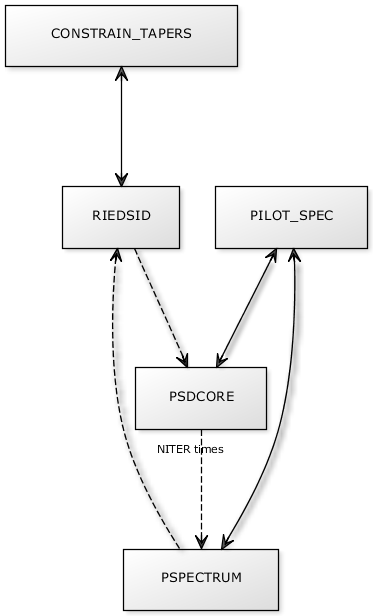
\includegraphics[width=0.6\textwidth]{yuml_d.png}%%
 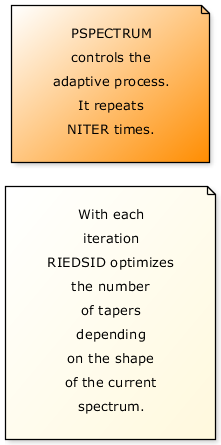
\includegraphics[width=0.4\textwidth]{yuml_n.png}
 \caption{Simplified call graph for \rlp{}. The dashed lines show a
 simplified circuit
 in which the spectra and its tapers make during the iterative process.}
 \label{fig:calls}
\end{figure}

%\section{Acknowledgements}

\section{Session Info}
\begin{knitrout}
\definecolor{shadecolor}{rgb}{0.969, 0.969, 0.969}\color{fgcolor}\begin{kframe}
\begin{alltt}
\hlfunctioncall{sessionInfo}()
\end{alltt}
\begin{verbatim}
## R version 2.15.2 (2012-10-26)
## Platform: x86_64-apple-darwin9.8.0/x86_64 (64-bit)
## 
## locale:
## [1] C
## 
## attached base packages:
##  [1] parallel  datasets  grDevices grid      graphics  tools     stats    
##  [8] utils     methods   base     
## 
## other attached packages:
##  [1] ggplot2_0.9.3      signal_0.7-2       MASS_7.3-22       
##  [4] RColorBrewer_1.0-5 RSEIS_3.0-9        Rwave_2.0         
##  [7] RPMG_2.1-4         rlpSpec_0.1-0      fftw_1.0-3        
## [10] knitr_0.9         
## 
## loaded via a namespace (and not attached):
##  [1] Peaks_0.2        colorspace_1.2-0 dichromat_1.2-4  digest_0.6.0    
##  [5] evaluate_0.4.3   formatR_0.7      gtable_0.1.2     labeling_0.1    
##  [9] lattice_0.20-10  munsell_0.4      plyr_1.8         proto_0.3-10    
## [13] reshape2_1.2.2   scales_0.2.3     stringr_0.6.2    zoo_1.7-9
\end{verbatim}
\end{kframe}
\end{knitrout}


%%
%\pagebreak
\bibliographystyle{apalike} %plainnat}
\bibliography{REFS}
\end{document}
